\chapter{Specifikacija programske potpore}

\section{Funkcionalni zahtjevi}

%\textbf{\textit{dio 1. revizije}}\\

%\textit{Navesti \textbf{dionike} koji imaju %\textbf{interes u ovom sustavu} ili  \textbf{su %nositelji odgovornosti}. To su prije svega %korisnici, ali i administratori sustava, %naručitelji, razvojni tim.}\\

%\textit{Navesti \textbf{aktore} koji izravno \textbf{koriste} ili \textbf{komuniciraju sa sustavom}. Oni mogu imati inicijatorsku ulogu, tj. započinju određene procese u sustavu ili samo sudioničku ulogu, tj. obavljaju određeni posao. Za svakog aktora navesti funkcionalne zahtjeve koji se na njega odnose.}\\


\noindent \textbf{Dionici:}

\begin{packed_enum}
	
	\item Vlasnik (naručitelj)
	\item Vlasnici kućnih ljubimaca				
	\item Ljudi koji pomažu u potrazi
	\item Skloništa za životinje
	\item Razvojni tim
	
\end{packed_enum}

\noindent \textbf{Aktori i njihovi funkcionalni zahtjevi:}


\begin{packed_enum}
	\item  \underbar{Neregistrirani korisnik (inicijator) može:}
	
	\begin{packed_enum}
		
		\item registrirati se, stvoriti novi korisnički račun za koje je potrebno unijeti ime, prezime, korisničko ime, lozinku, adresu e-pošte, broj telefona
		\item pregledavati i pretraživati aktivne oglase
		\item odabrati oglas za detaljniji pregled informacija o kućnom ljubimcu i pregled komunikacije oko kućnog ljubimca
		
		
	\end{packed_enum}
	
	\item  \underbar{Vlasnik kućnog ljubimca (inicijator) može:}
	
	\begin{packed_enum}
		
		\item izbrisati korisnički račun
		\item pregledavati i mijenjati osobne podatke
		\item pregledavati aktivne i neaktivne oglase
		\item postaviti oglas o nestalom kućnom ljubimcu za koji je potrebno unijeti vrstu, ime na koje se odaziva, datum i sat nestanka, lokaciju nestanka, boju, starost, tekstni opis i slike (do 3)
		\item sudjelovati u komunikaciji o nestalom kućnom ljubimcu
		\begin{packed_enum}
			
			\item sudjelovati slanjem tekstne poruke
			\item sudjelovati slanjem slike
			\item sudjelovati slanjem geolokacije
			
		\end{packed_enum}
		\item ukloniti oglas o nestalom kućnom ljubimcu
		\item izmjenjivati oglas o nestalom kućnom ljubimcu
		
		
	\end{packed_enum}
	
	\item  \underbar{Sudionik u potrazi (inicijator) može:}
	
	\begin{packed_enum}
		
		\item izbrisati korisnički račun
		\item pregledavati i mijenjati osobne podatke
		\item pregledavati aktivne i neaktivne oglase
		\item sudjelovati u komunikaciji o nestalom kućnom ljubimcu
		\begin{packed_enum}
			
			\item sudjelovati slanjem tekstne poruke
			\item sudjelovati slanjem slike
			\item sudjelovati slanjem geolokacije
			
		\end{packed_enum}
		
	\end{packed_enum}
	\item  \underbar{Sklonište za životinje (inicijator) može:}
	
	\begin{packed_enum}
		
		\item izbrisati korisnički račun
		\item pregledavati aktivne i neaktivne oglase
		\item postaviti oglas o pronađenoj životinji
		\item sudjelovati u komunikaciji o nestalom kućnom ljubimcu
		\begin{packed_enum}
			
			\item sudjelovati slanjem tekstne poruke
			\item sudjelovati slanjem slike
			\item sudjelovati slanjem geolokacije
			
		\end{packed_enum}
		
		
	\end{packed_enum}
	
	\item  \underbar{Baza podataka (sudionik) može:}
	
	\begin{packed_enum}
		
		\item pohraniti podatke o korisnicima
		\item pohraniti podatke o kućnim ljubimcima (oglase)
		
		
		
	\end{packed_enum}
	
\end{packed_enum}

\eject 



\subsection{Obrasci uporabe}

%\textbf{\textit{dio 1. revizije}}

%\subsubsection{Opis obrazaca uporabe}
%\textit{Funkcionalne zahtjeve razraditi u obliku obrazaca uporabe. Svaki obrazac je potrebno razraditi prema donjem predlošku. Ukoliko u nekom koraku može doći do odstupanja, potrebno je to odstupanje opisati i po mogućnosti ponuditi rješenje kojim bi se tijek obrasca vratio na osnovni tijek.}\\


\noindent \underbar{\textbf{UC1 - Pregled aktivnih oglasa}}
\begin{packed_item}
	
	\item \textbf{Glavni sudionik: }Korisnik
	\item  \textbf{Cilj:} Pregledati oglase o nestalim kućnim ljubimcima
	\item  \textbf{Sudionici:} Baza podataka
	\item  \textbf{Preduvjet:} -
	\item  \textbf{Opis osnovnog tijeka:}
	
	\item[] \begin{packed_enum}
		
		\item Aktivni oglasi su prikazani prilikom učitavanja aplikacije
		\item Korisnik odabire oglas za više informacija
		\item Prikazuju se informacije i komunikacija o nestalom kućnom ljubimcu

	\end{packed_enum}
	
\end{packed_item}

\noindent \underbar{\textbf{UC2 - Registracija}}
\begin{packed_item}
	
	\item \textbf{Glavni sudionik: }Korisnik
	\item  \textbf{Cilj:} Stvoriti korisnički račun za pristup sustavu
	\item  \textbf{Sudionici:} Baza podataka
	\item  \textbf{Preduvjet:} -
	\item  \textbf{Opis osnovnog tijeka:}
	
	\item[] \begin{packed_enum}
		
		\item Korisnik odabire opciju za registraciju
		\item Korisnik unosi potrebne korisničke podatke
		\item Korisnik prima obavijest o uspješnoj registraciji

	\end{packed_enum}
	
	\item  \textbf{Opis mogućih odstupanja:}
	
	\item[] \begin{packed_item}
		
		\item[2.a] Odabir već zauzetog korisničkog imena i/ili e-maila, unos korisničkog podatka u nedozvoljenom formatu ili unos neispravnoga e-maila
		
		\item[] \begin{packed_enum}
			
			\item Sustav obavještava korisnika o pogrešnom unosu podataka i vraća ga na stranicu za registraciju
			\item Korisnik mijenja potrebne podatke te završava unos ili odustaje od registracije
			
		\end{packed_enum}

		
	\end{packed_item}
\end{packed_item}



\noindent \underbar{\textbf{UC3 - Prijava u sustav}}
\begin{packed_item}
	
	\item \textbf{Glavni sudionik: }Registrirani korisnik
	\item  \textbf{Cilj:} Dobiti pristup korisničkom sučelju
	\item  \textbf{Sudionici:} Baza podataka
	\item  \textbf{Preduvjet:}  Registracija
	\item  \textbf{Opis osnovnog tijeka:}
	
	\item[] \begin{packed_enum}
		
		\item Unos korisničkog imena i lozinke
		\item Potvrda o ispravnosti unesenih podataka
		\item Pristup korisničkim funkcijama

	\end{packed_enum}
	
	\item  \textbf{Opis mogućih odstupanja:}
	
	\item[] \begin{packed_item}
		
		\item[2.a] Neispravno korisničko ime/lozinka
		\item[] \begin{packed_enum}
			
			\item Sustav obavještava korisnika o neuspjeloj prijavi i vraća ga na stranicu za prijavu u sustav
			\item Korisnik unosi ispravne podatke i uspješno se prijavljuje u sustav
			
		\end{packed_enum}
		
	\end{packed_item}
\end{packed_item}

\noindent \underbar{\textbf{UC4 - Pregled osobnih podataka}}
\begin{packed_item}
	
	\item \textbf{Glavni sudionik: }Registrirani korisnik
	\item  \textbf{Cilj:} Pregledati osobne podatke
	\item  \textbf{Sudionici:} Baza podataka
	\item  \textbf{Preduvjet:} Korisnik je prijavljen
	\item  \textbf{Opis osnovnog tijeka:}
	
	\item[] \begin{packed_enum}
		
		\item Korisnik odabire opciju ”Osobni podatci”
		\item Aplikacija prikazuje osobne podatke korisnika

	\end{packed_enum}
	
\end{packed_item}

\noindent \underbar{\textbf{UC5 - Promjena osobnih podataka}}
\begin{packed_item}
	
	\item \textbf{Glavni sudionik: }Registrirani korisnik
	\item  \textbf{Cilj:} Promijeniti osobne podatke
	\item  \textbf{Sudionici:} Baza podataka
	\item  \textbf{Preduvjet:} Korisnik je prijavljen
	\item  \textbf{Opis osnovnog tijeka:}
	
	\item[] \begin{packed_enum}
		
		\item Korisnik odabere opciju za promjenu podataka
		\item Korisnik upisuje nove osobne podatke
		\item Korisnik sprema promjene
		\item Baza podataka sprema nove podatke
	\end{packed_enum}
	
	\item  \textbf{Opis mogućih odstupanja:}
	
	\item[] \begin{packed_item}
		
		\item[3.a] Korisnik promijeni svoje osobne podatke, ali ne odabere opciju ”Spremi promjenu”
		
		\item[] \begin{packed_enum}
			
			\item Sustav obavještava korisnika da nije spremio podatke prije izlaska iz prozora
			
		\end{packed_enum}
		
		
	\end{packed_item}
\end{packed_item}

\noindent \underbar{\textbf{UC6 - Brisanje korisničkog računa}}
\begin{packed_item}
	
	\item \textbf{Glavni sudionik: }Registrirani korisnik
	\item  \textbf{Cilj:} Izbrisati svoj korisnički račun
	\item  \textbf{Sudionici:} Baza podataka
	\item  \textbf{Preduvjet:} Korisnik je prijavljen
	\item  \textbf{Opis osnovnog tijeka:}
	
	\item[] \begin{packed_enum}
		
		\item Korisnik pregledava osobne podatke
		\item Otvara se stranica s osobnim podacima korisnika
		\item Korisnik odabire opciju „Izbriši račun“
		\item Korisnički račun briše se iz baze podataka
		\item Otvara se stranica za registraciju
	\end{packed_enum}
	
\end{packed_item}

\noindent \underbar{\textbf{UC7 - Postavljanje oglasa}}
\begin{packed_item}
	
	\item \textbf{Glavni sudionik: }Registrirani korisnik
	\item  \textbf{Cilj:} Postavljanje oglasa o nestalom kućnom ljubimcu
	\item  \textbf{Sudionici:} Baza podataka
	\item  \textbf{Preduvjet:} Korisnik je prijavljen
	\item  \textbf{Opis osnovnog tijeka:}
	
	\item[] \begin{packed_enum}
		
		\item Korisnik odabire opciju "Novi oglas"
		\item Korisnik unosi podatke o nestalom kućnom ljubimcu
		\item Korisnik odabire opciju "Postavi oglas"
	\end{packed_enum}
	
	\item  \textbf{Opis mogućih odstupanja:}
	
	\item[] \begin{packed_item}
		
		\item[3.a] Korisnik ne unosi obvezne podatke o ljubimcu
		\item[] \begin{packed_enum}
			
			\item Sustav obavještava korisnika da nisu uneseni svi potrebni podaci
			\item Korisnik unosi sve podatke
			\item Korisnik postavlja oglas
		
		
			\end{packed_enum}
			
			
		\item[3.b] Korisnik odustaje od postavljanja oglasa
		\item[] \begin{packed_enum}
			\item Sustav obavještava korisnika da oglas neće biti postavljen
			\item Prikazuje se početna stranica
		\end{packed_enum}
		
		
	\end{packed_item}
\end{packed_item}

\noindent \underbar{\textbf{UC8 - Moji oglasi}}
\begin{packed_item}
	
	\item \textbf{Glavni sudionik: }Registrirani korisnik
	\item  \textbf{Cilj:} Pregledati listu oglasa koje je postavio korisnik
	\item  \textbf{Sudionici:} Baza podataka
	\item  \textbf{Preduvjet:} Korisnik je prijavljen u sustav
	\item  \textbf{Opis osnovnog tijeka:}
	
	\item[] \begin{packed_enum}
		
		\item Korisnik odabire opciju "Moji oglasi"
		\item Aplikacija prikazuje listu oglasa koje je postavio korisnik

	\end{packed_enum}
	
	\item  \textbf{Opis mogućih odstupanja:}
	
	\item[] \begin{packed_item}
		
		\item[2.a] Korisnik nema postavljene oglase
		\item[] \begin{packed_enum}
			
			\item Sustav obavještava korisnika da još nije postavio oglas
			
		\end{packed_enum}
		
		
	\end{packed_item}
\end{packed_item}

\noindent \underbar{\textbf{UC9 - Izmjena kategorije oglasa}}
\begin{packed_item}
	
	\item \textbf{Glavni sudionik: }Registrirani korisnik
	\item  \textbf{Cilj:} Promijeniti kategoriju oglasa
	\item  \textbf{Sudionici:} Baza podataka
	\item  \textbf{Preduvjet:} Korisnik je prijavljen u sustav
	\item  \textbf{Opis osnovnog tijeka:}
	
	\item[] \begin{packed_enum}
		
		\item Korisnik odabire opciju "Moji oglasi"
		\item Odabire oglas kojem želi promijeniti kategoriju
		\item Odabire opciju "Uredi"
		\item Korisnik odabire jednu od ponuđenih kategorija
		\item Korisnik odabire opciju "Spremi"
		\item Oglas je promijenjen
	\end{packed_enum}
	
	\item  \textbf{Opis mogućih odstupanja:}
	
	\item[] \begin{packed_item}
		
		\item[2.a] UC8
		
		\item[5.a] Korisnik ne odabire opciju "Spremi"
		\item[] \begin{packed_enum}
			
			\item Oglas ostaje nepromijenjen
			
		\end{packed_enum}
		
	\end{packed_item}
\end{packed_item}

\noindent \underbar{\textbf{UC10 - Uklanjanje oglasa}}
\begin{packed_item}
	
	\item \textbf{Glavni sudionik: }Registrirani korisnik
	\item  \textbf{Cilj:} Ukloniti oglas
	\item  \textbf{Sudionici:} Baza podataka
	\item  \textbf{Preduvjet:} Korisnik je prijavljen
	\item  \textbf{Opis osnovnog tijeka:}
	
	\item[] \begin{packed_enum}
		
		\item Korisnik odabire opciju "Moji oglasi"
		\item Odabire oglas kojeg želi izbrisati
		\item Korisnik odabire opciju "Izbriši"
	\end{packed_enum}
	
	\item  \textbf{Opis mogućih odstupanja:}
	
	\item[] \begin{packed_item}
		
		\item[3.a] korisnik odustaje od brisnja oglasa
		\item[] \begin{packed_enum}
			
			\item Korisnik odabire opciju "Odustani"
			\item Aplikacija prikazuje listu korisnikovih oglasa
			
		\end{packed_enum}
		
		
	\end{packed_item}
\end{packed_item}

\noindent \underbar{\textbf{UC11 - Komunikacija}}
\begin{packed_item}
	
	\item \textbf{Glavni sudionik: }Registrirani korisnik
	\item  \textbf{Cilj:} Kominikacija oko pronalaska kućnog ljubimca
	\item  \textbf{Sudionici:} Baza podataka
	\item  \textbf{Preduvjet:} Korisnik je prijavljen
	\item  \textbf{Opis osnovnog tijeka:}
	
	\item[] \begin{packed_enum}
		
		\item Korisnik odabire oglas o kućnom ljubimcu
		\item Korisnik odabire opciju "Poruke"
		\item Aplikacija prikazuje poruke vezane za komunikaciju oko potrage za kućnim ljubimcem

	\end{packed_enum}
	

\end{packed_item}

\noindent \underbar{\textbf{UC12 - Slanje poruke}}
\begin{packed_item}
	
	\item \textbf{Glavni sudionik: }Registrirani korisnik
	\item  \textbf{Cilj:} Poslati poruku s informacijama o kućnom ljubimcu
	\item  \textbf{Sudionici:} Baza podataka
	\item  \textbf{Preduvjet:} Korisnik je prijavljen
	\item  \textbf{Opis osnovnog tijeka:}
	
	\item[] \begin{packed_enum}
		
		\item UC11
		\item Korisnik odabire opciju "Pošalji poruku"
		\item Korisnik unosi poruku
		\item Korisnik odabire opciju "Pošalji" i šalje poruku
		
	\end{packed_enum}
	
	\item  \textbf{Opis mogućih odstupanja:}
	
	\item[] \begin{packed_item}
		
		\item[3.a] korisnik odustaje od slanja poruke
		\item[] \begin{packed_enum}
			
			\item Korisnik odabire opciju "Odustani"
			\item Aplikacija prikazuje poruke vezane za komunikaciju oko potrage za kućnim ljubimcem
			
		\end{packed_enum}
		
		
	\end{packed_item}
\end{packed_item}

\noindent \underbar{\textbf{UC13 - Slanje slike}}
\begin{packed_item}
	
	\item \textbf{Glavni sudionik: }Registrirani korisnik
	\item  \textbf{Cilj:} Poslati sliku u poruci
	\item  \textbf{Sudionici:} Baza podataka
	\item  \textbf{Preduvjet:} Korisnik je prijavljen
	\item  \textbf{Opis osnovnog tijeka:}
	
	\item[] \begin{packed_enum}
		
		\item UC11
		\item Korisnik odabire opciju "Pošalji poruku"
		\item Korisnik odabire opciju "Dodaj sliku u privitak"
		\item Korisnik odabire sliku
		\item Korisnik odabire opciju "Pošalji" i šalje poruku
		
		
	\end{packed_enum}
	
	\item  \textbf{Opis mogućih odstupanja:}
	
	\item[] \begin{packed_item}
		
		\item[4.a] UC12 3.a
		\item[5.a] UC12 3.a
		
		
	\end{packed_item}
\end{packed_item}

\noindent \underbar{\textbf{UC14 - Slanje geolokacije}}
\begin{packed_item}
	
	\item \textbf{Glavni sudionik: }Registrirani korisnik
	\item  \textbf{Cilj:} Poslati geolokaciju u poruci
	\item  \textbf{Sudionici:} Baza podataka
	\item  \textbf{Preduvjet:} Korisnik je prijavljen
	\item  \textbf{Opis osnovnog tijeka:}
	
	\item[] \begin{packed_enum}
		
		\item UC11
		\item Korisnik odabire opciju "Pošalji poruku"
		\item Korisnik odabire opciju "Dodaj geolokaciju"
		\item Korisnik odabire geolokaciju
		\item Korisnik odabire opciju "Pošalji" i šalje poruku
		
	\end{packed_enum}
	
	\item  \textbf{Opis mogućih odstupanja:}
	
	\item[] \begin{packed_item}
		
		\item[4.a] UC12 3.a
		\item[5.a] UC12 3.a
		
		
	\end{packed_item}
\end{packed_item}

\noindent \underbar{\textbf{UC15 - Pretraživanje oglasa}}
\begin{packed_item}
	
	\item \textbf{Glavni sudionik: } Korisnik
	\item  \textbf{Cilj:} Pretražiti oglas po kategoriji
	\item  \textbf{Sudionici:} Baza podataka
	\item  \textbf{Preduvjet:} -
	\item  \textbf{Opis osnovnog tijeka:}
	
	\item[] \begin{packed_enum}
		
		\item Korisnik odabire kategoriju po kojoj želi pretraživati (jednu ili više)
		\item Korisnik odabire opciju "Pretraži"
		\item Aplikacija prikazuje filtrirane oglase
		
	\end{packed_enum}
	
	\item  \textbf{Opis mogućih odstupanja:}
	
	\item[] \begin{packed_item}
		
		\item[1.a] Korisnik unosi nevaljani datum, grad ili ulicu
		\item[] \begin{packed_enum}
			
			\item Sustav javlja korisniku da je unesen nevaljani podatak za pretragu
			
			
		\end{packed_enum}
		
		
	\end{packed_item}
\end{packed_item}

\subsubsection{Dijagrami obrazaca uporabe}

%\textit{Prikazati odnos aktora i obrazaca uporabe odgovarajućim UML dijagramom. Nije nužno nacrtati sve na jednom dijagramu. Modelirati po razinama apstrakcije i skupovima srodnih funkcionalnosti.}
%\eject		

\begin{figure}[H]
	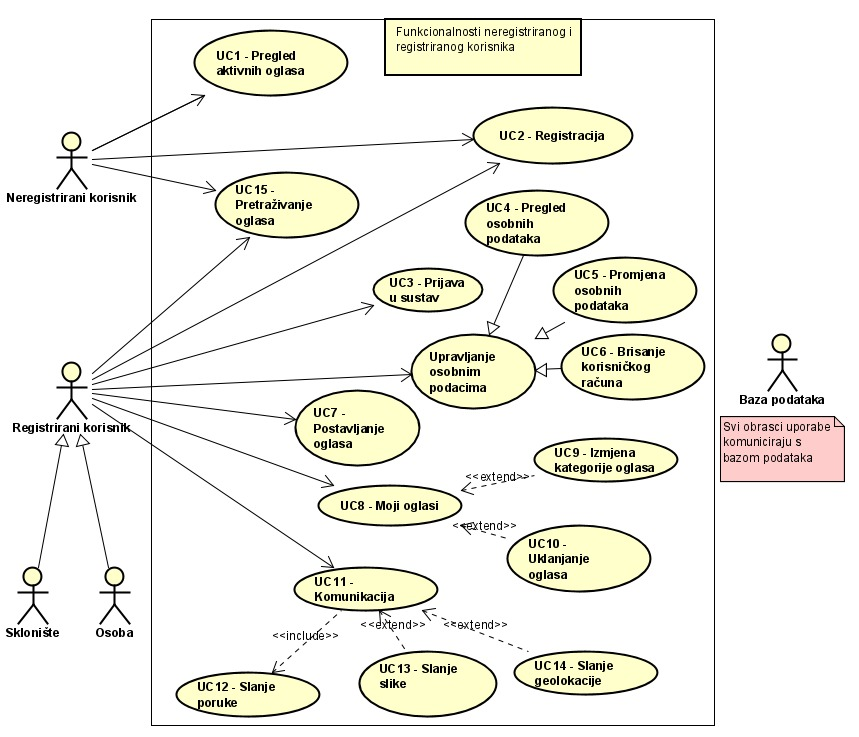
\includegraphics[width=\textwidth]{Dijagram_obrasca_uporabe.JPEG} %veličina u odnosu na širinu linije
	\caption{Dijagram obrasca uporabe, funkcionalnosti neregistriranog i registriranog korisnika}
	\label{fig:promjene6} %label mora biti drugaciji za svaku sliku
\end{figure}

\pagebreak

\subsection{Sekvencijski dijagrami}

%\textbf{\textit{dio 1. revizije}}\\

%\textit{Nacrtati sekvencijske dijagrame koji modeliraju najvažnije dijelove sustava (max. 4 dijagrama). Ukoliko postoji nedoumica oko odabira, razjasniti s asistentom. Uz svaki dijagram napisati detaljni opis dijagrama.}
%\eject

\noindent {\textbf{Obrazac uporabe UC3 - Prijava u sustav}}


\noindent{Korisnik odabire opciju "Prijavi se". Sustav prikazuje formu za prijavu, te korisnik unosi potrebne podatke. Sustav provjerava postoje li uneseni podaci u bazi podataka. Ako su uneseni podaci ispravni, sustav obavještava korisnika da je prijava uspjela te mu omogućava pristup korisničkim funkcijama. U slučaju unosa pogrešnih podataka sustav obavještava korisnika o pogrešci, te se ponovno prikazuje forma za prijavu.}
	
	
\begin{figure}[H]
	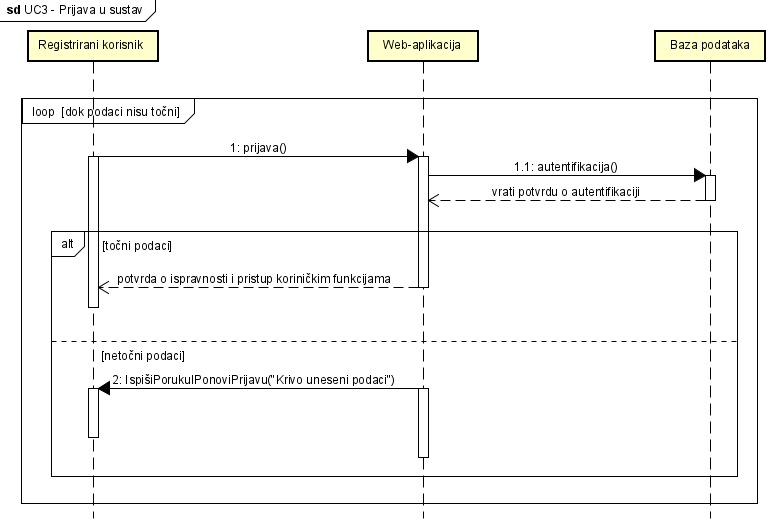
\includegraphics[width=\textwidth]{sekvencijski_dijagram_prijava_u_sustav.JPEG} %veličina u odnosu na širinu linije
	\caption{Sekvencijski dijagram za UC3}
	\label{fig:promjene3} %label mora biti drugaciji za svaku sliku
\end{figure}

\pagebreak

\noindent {\textbf{Obrazac uporabe UC7 - Postavljanje oglasa}}

\noindent{Korisnik odabire opciju "Novi oglas". Sustav prikazuje formu za unos podataka o izgubljenom kućnom ljubimcu. Korisnik unosi podatke, te odabire opciju "Spremi". Sustav provjerava u bazi podataka jesu li uneseni svi potrebni podaci. Baza podataka vraća provjeru sustavu, te ako su uneseni svi potrebni podaci za postavljanje oglasa, oglas se pohranjuje u bazu podataka i sustav obavještava korisnika da je oglas uspješno spremljen. U suprotnom, sustav obavještava korisnika da nisu uneseni svi potrebni podaci.}

\begin{figure}[H]
	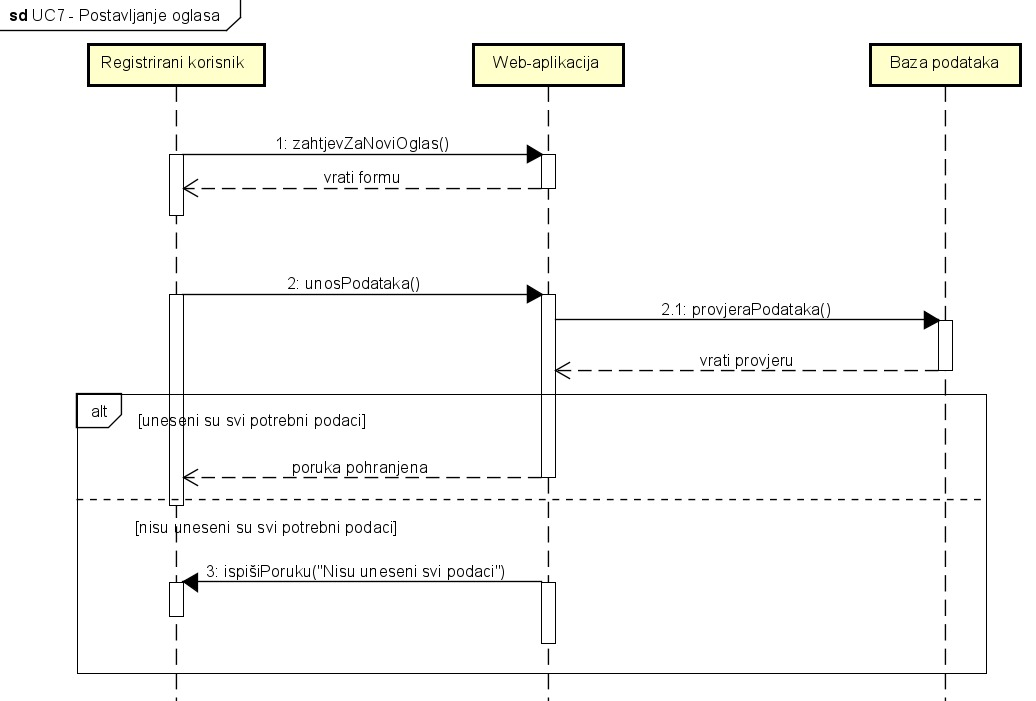
\includegraphics[width=\textwidth]{sekvencijski_dijagram_postavljanje_oglasa.JPEG} %veličina u odnosu na širinu linije
	\caption{Sekvencijski dijagram za UC7}
	\label{fig:promjen43} %label mora biti drugaciji za svaku sliku
\end{figure}

\pagebreak

\noindent {\textbf{Obrazac uporabe UC12 - Slanje poruke}}

\noindent{Kako bi korisnik poslao poruku, najprije mora odabrati oglas na kojem želi ostaviti poruku. Nakon odabira oglasa iz baze podataka se dohvaćaju podaci vezani za taj oglas. Sustav prikazuje oglas (podatke o nestalom kućnom ljubimcu). Korisnik odabire opciju "Prikaži poruke", te se iz baze podataka dohvaćaju sve dosadašnje poruke vezane za nestalog kućnog ljubimca. Sustav sada, uz podatke o ljubimcu, prikazuje i svu dosadašnju komunikaciju vezanu za nestalog kućnog ljubimca. Korisnik odabire opciju "Nova poruka" i unosi željeni tekst, te opcionalno sliku ili geolokaciju. Nakon što korisnik odabere opciju "Pošalji poruku", poruka se upisuje u bazu podataka. Nakon što je poruka uspješno upisana u bazu podataka, sustav obavještava korisnika da je poruka poslana.}

\begin{figure}[H]
	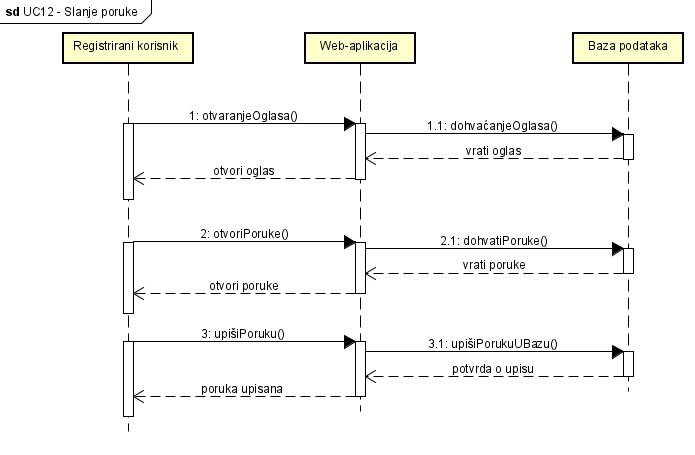
\includegraphics[width=\textwidth]{sekvencijski_dijagram_slanje_poruka.JPEG} %veličina u odnosu na širinu linije
	\caption{Sekvencijski dijagram za UC12}
	\label{fig:promjene5} %label mora biti drugaciji za svaku sliku
\end{figure}


\pagebreak

\section{Ostali zahtjevi}

%\textbf{\textit{dio 1. revizije}}\\

%\textit{Nefunkcionalni zahtjevi i zahtjevi domene primjene dopunjuju funkcionalne zahtjeve. Oni opisuju \textbf{kako se sustav treba ponašati} i koja \textbf{ograničenja} treba poštivati (performanse, korisničko iskustvo, pouzdanost, standardi kvalitete, sigurnost...). Primjeri takvih zahtjeva u Vašem projektu mogu biti: podržani jezici korisničkog sučelja, vrijeme odziva, najveći mogući podržani broj korisnika, podržane web/mobilne platforme, razina zaštite (protokoli komunikacije, kriptiranje...)... Svaki takav zahtjev potrebno je navesti u jednoj ili dvije rečenice.}

\begin{packed_item}
	\item Sustav treba omogućiti rad više korisnika u stvarnom vremenu
	\item Neispravno korištenje korisničkog sučelja ne smije narušiti funkcionalnost sustava
	\item Aplikacija treba biti izvedena kao web aplikacija prilagođena za mobilne uređaje (responzivna)
	\item Korisničko sučelje i sustav moraju podržavati hrvatsku abecedu (dijakritičke znakove) pri unosu i prikazu tekstualnog sadržaja
	\item Sustav treba biti jednostavan za korištenje
	
\end{packed_item}

